\chapter{Results and evaluation} \label{chap:results}
\section{Table of all results}
e
\section{Accuracy of Iteration 1}
As mentioned in \autoref{ssec:iteration1layers}, various combinations of LSTM layers and Dense layers were tested,
each with various sizes. The results of all of the models can be seen in \autoref{fig:iteration1_train_accuracy}
and \autoref{fig:iteration1_all_accuracy}.\\
The results of the best model can be seen in \autoref{fig:iteration1_best_accuracy}

\subsection{Accuracies of all tests}
In the charts below, each line represents a combination of different layer types and sizes of the Dense and LSTM layers of the chart.
For both the training and validation accuracy charts, each line has a corresponding line in the loss charts with the same colour.
There are 16 lines in total for this iteration as there were 2 LSTM layer amounts, 2 Dense layer amounts,
2 LSTM layer sizes, and 2 Dense layer sizes in the tests.

\subsubsection{Training accuracies and losses}
\begin{figure}[ht]
    \centering
    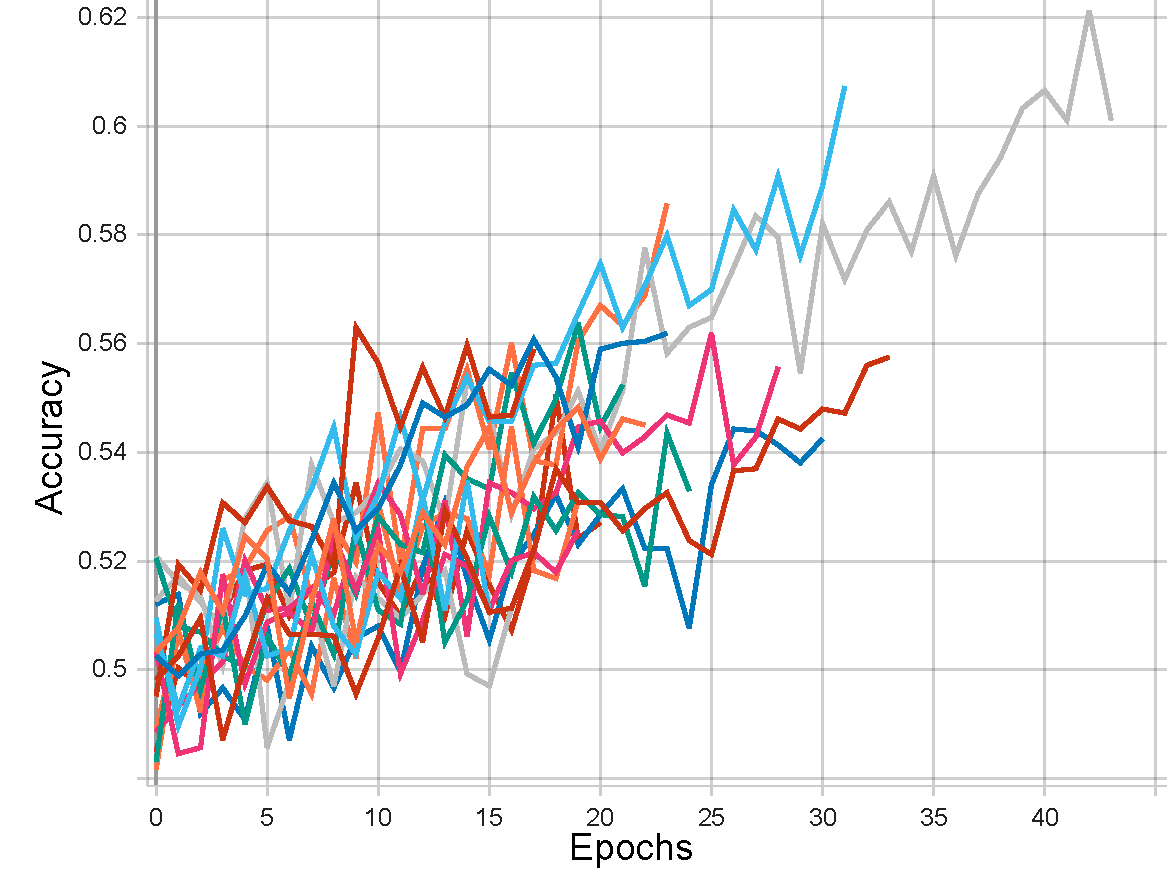
\includegraphics[width=0.95\columnwidth]{figures/results/lstm/lstm_all_acc_t.pdf}
    \caption[Training accuracies for Iteration 1]{Figure of all training accuracies of the combinations of LSTM Layers and Dense Layers in Iteration 1}
    \label{fig:iteration1_train_accuracy}
\end{figure}
\FloatBarrier
\begin{figure}[ht]
    \centering
    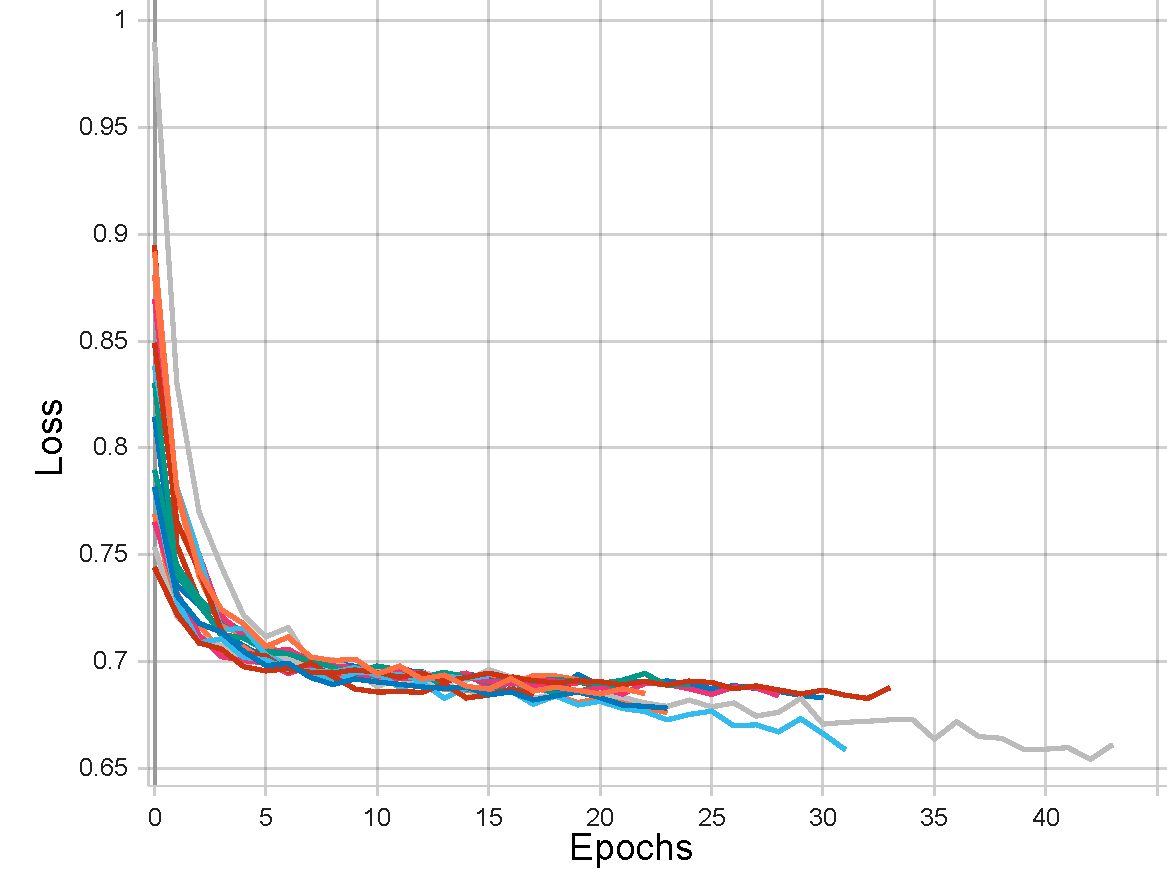
\includegraphics[width=0.95\columnwidth]{figures/results/lstm/lstm_all_loss_t.pdf}
    \caption[Training losses for Iteration 1]{Figure of all training losses of the combinations of LSTM Layers and Dense Layers in Iteration 1}
    \label{fig:iteration1_train_loss}
\end{figure}
\FloatBarrier

\subsubsection{Validation accuracies and losses}
\begin{figure}[ht]
    \centering
    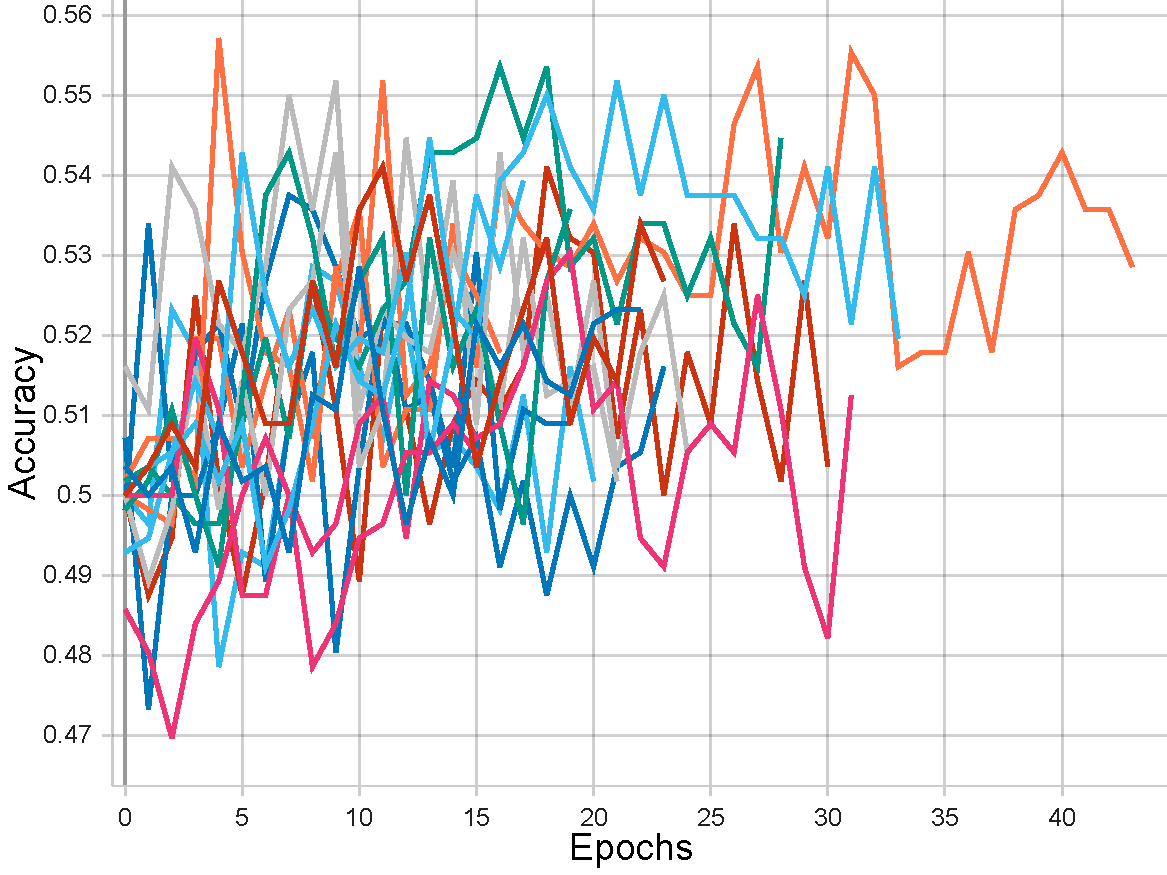
\includegraphics[width=0.95\columnwidth]{figures/results/lstm/lstm_all_acc.pdf}
    \caption[Validation accuracies for Iteration 1]{Figure of all validation accuracies of the combinations of LSTM Layers and Dense Layers in Iteration 1}
    \label{fig:iteration1_all_accuracy}
\end{figure}
\FloatBarrier
\begin{figure}[ht]
    \centering
    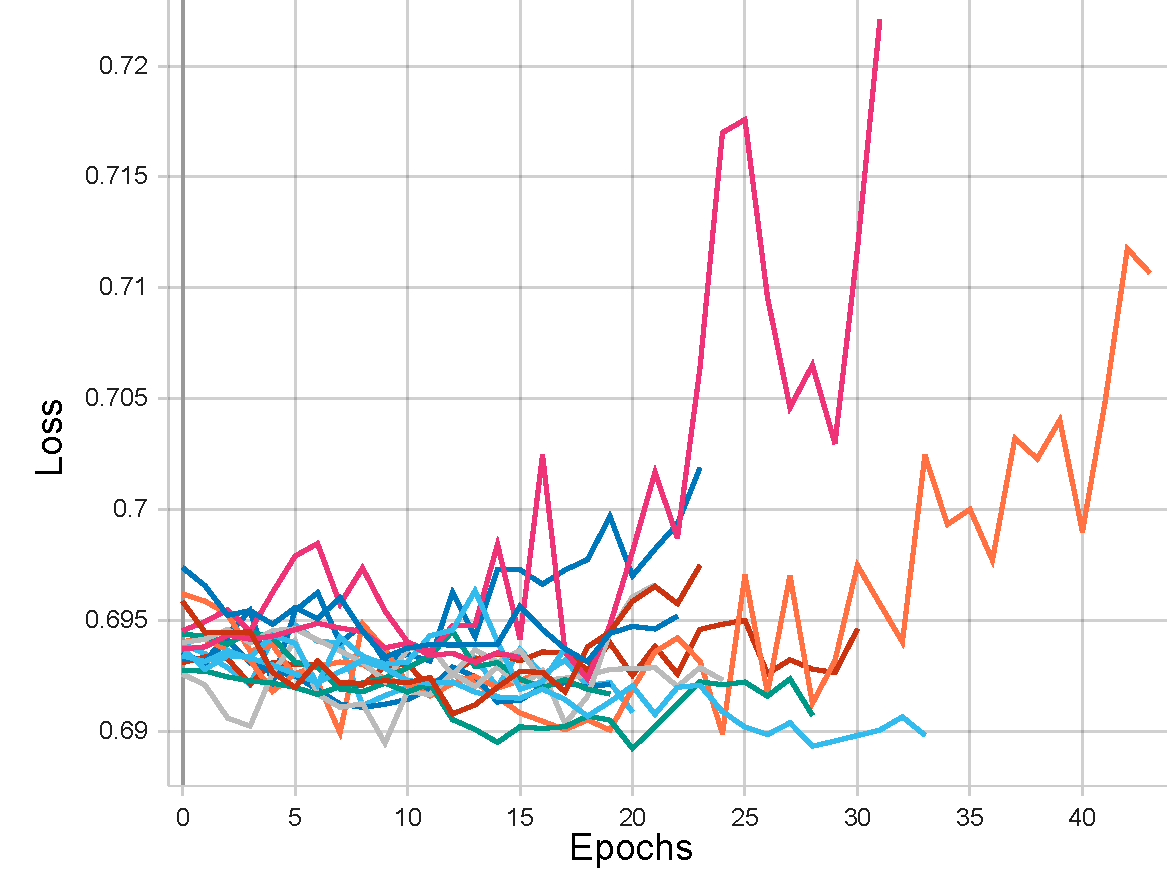
\includegraphics[width=0.95\columnwidth]{figures/results/lstm/lstm_all_loss.pdf}
    \caption[Validation losses for Iteration 1]{Figure of all validation losses of the combinations of LSTM Layers and Dense Layers in Iteration 1}
    \label{fig:iteration1_all_loss}
\end{figure}
\FloatBarrier

There are varying degrees of success with different combinations of layers; some do not improve in accuracy and others do.
The validation losses using the sparse categorical loss function as described earlier in \autoref{sec:model_fitting}
were used to help identify which models had the lowest error rate; and as an increasing validation
loss is an indicator of overfitting, it was used to filter models showing overfitting.

\subsection{Accuracies of the best result}
\begin{figure}[ht]
    \centering
    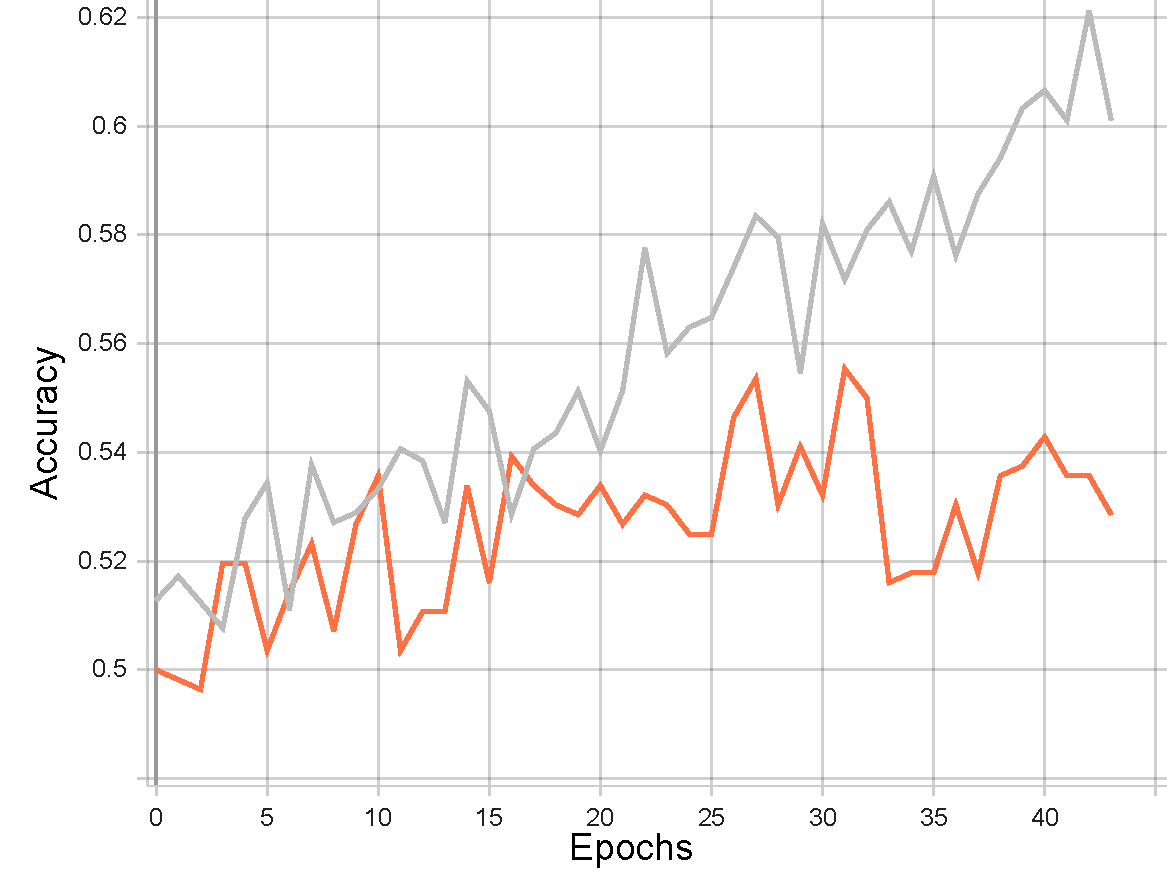
\includegraphics[width=0.95\columnwidth]{figures/results/lstm/lstm_2L64-2D32_acc.pdf}
    \caption[Best accuracy for Iteration 1]{Figure of the best accuracy of the combinations of LSTM Layers and Dense Layers in Iteration 1}
    \label{fig:iteration1_best_accuracy}
\end{figure}
\FloatBarrier
\begin{figure}[ht]
    \centering
    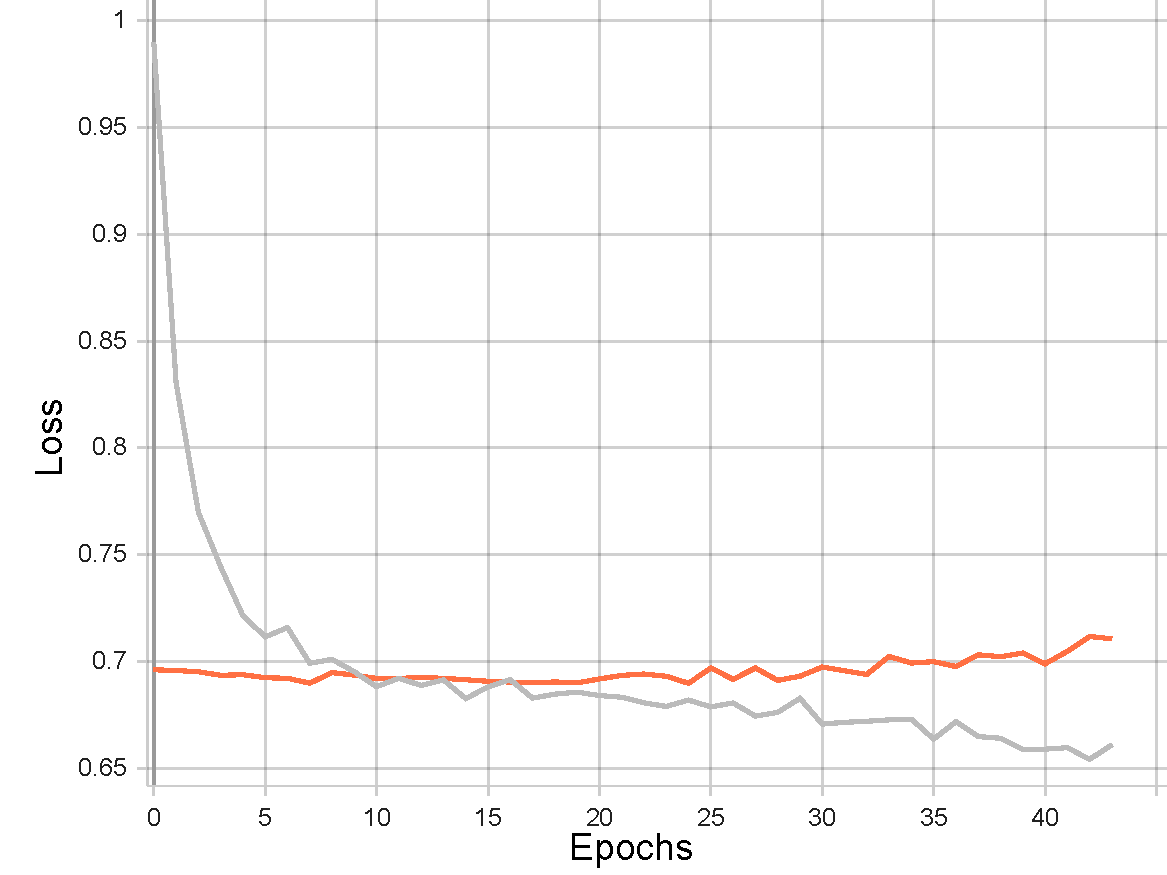
\includegraphics[width=0.95\columnwidth]{figures/results/lstm/lstm_2L64-2D32_loss.pdf}
    \caption[Best loss for Iteration 1]{Figure of the best loss of the combinations of LSTM Layers and Dense Layers in Iteration 1}
    \label{fig:iteration1_best_loss}
\end{figure}
\FloatBarrier
The best model found within this iteration was one with a two LSTM layers of size 64 followed
by the final Dense layer of size 2. The grey line represents the training set and the orange line represents
the validation set. The validation loss shows little overfitting as can be seen in
\autoref{fig:iteration1_best_loss}. At 31 epochs, the validation accuracy reaches its highest value of
55.54\% whilst the training accuracy reached above 57.18\%.
\subsection{Evaluation of iteration 1}
With a validation accuracy above 55\% it suggests that there is improvement above a random choice. It forms a good
basis for testing further AI models, specifically the CNN-LSTM hybrid model.
There are various limitations with regards to iteration 1. This iteration does not test various combinations of
input features nor does it test various sequence lengths. Furthermore, there could be another number of layers or
layer sizes that is better suited to the problem but unfortunately many have not been tested due to time constraints.

\section{Accuracy of Iteration 2}
As mentioned in \autoref{ssec:iteration2layers}, various combinations of Conv1D layers and Dense layers were tested,
each with various sizes. The results of all of the models can be seen in \autoref{fig:iteration2_train_accuracy}
and \autoref{fig:iteration2_all_accuracy}.\\
The results of the best model can be seen in \autoref{fig:iteration2_best_accuracy}

\subsection{Accuracies of all tests}
In the charts below, each line represents a combination of different layer types and sizes of the Dense and LSTM layers of the chart.
For both the training and validation accuracy charts, each line has a corresponding line in the loss charts with the same colour.
There are 16 lines in total for this iteration as there were 2 Conv1D layer amounts, 2 Dense layer amounts,
2 Conv1D layer sizes, and 2 Dense layer sizes in the tests.

\subsubsection{Training accuracies and losses}
\begin{figure}[ht]
    \centering
    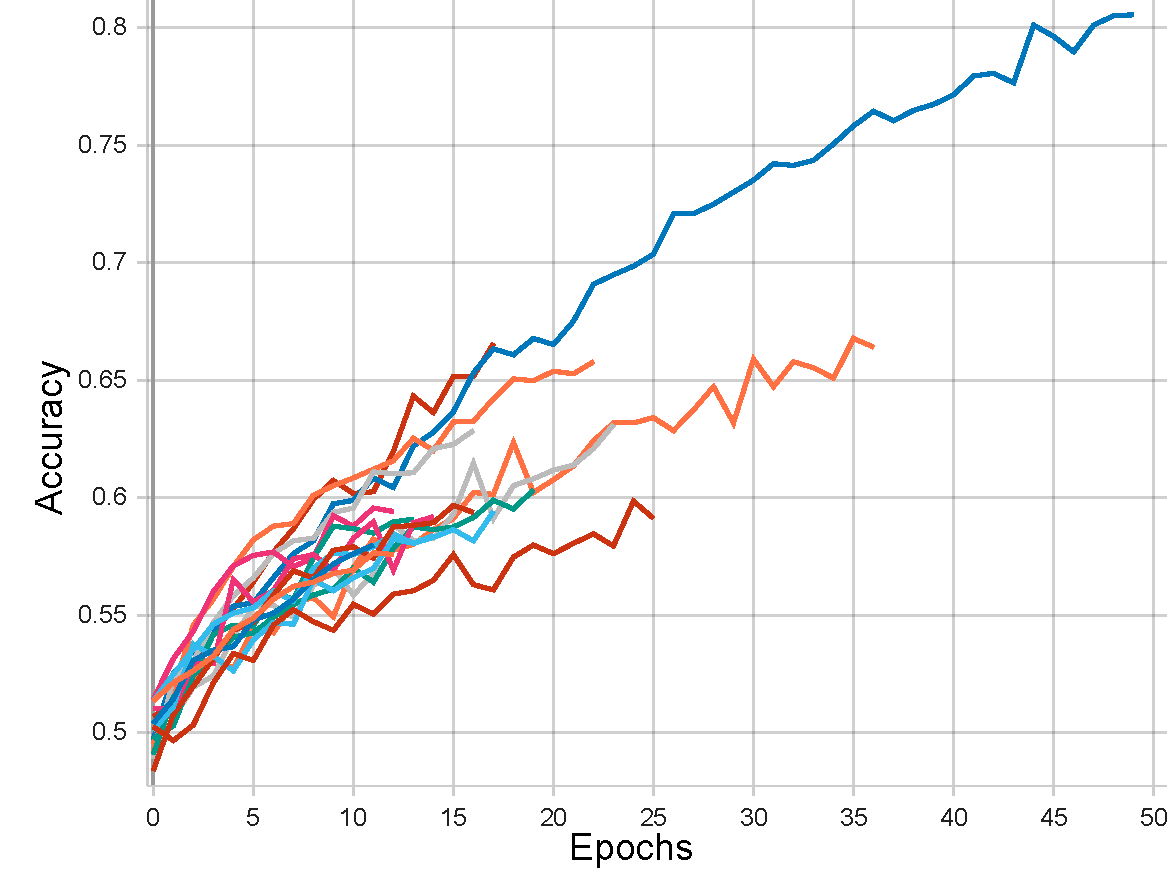
\includegraphics[width=0.95\columnwidth]{figures/results/cnn/cnn_all_acc_t.pdf}
    \caption[Training accuracies for Iteration 2]{Figure of all training accuracies of the combinations of Conv1D Layers and Dense Layers in Iteration 2}
    \label{fig:iteration2_train_accuracy}
\end{figure}
\FloatBarrier
\begin{figure}[ht]
    \centering
    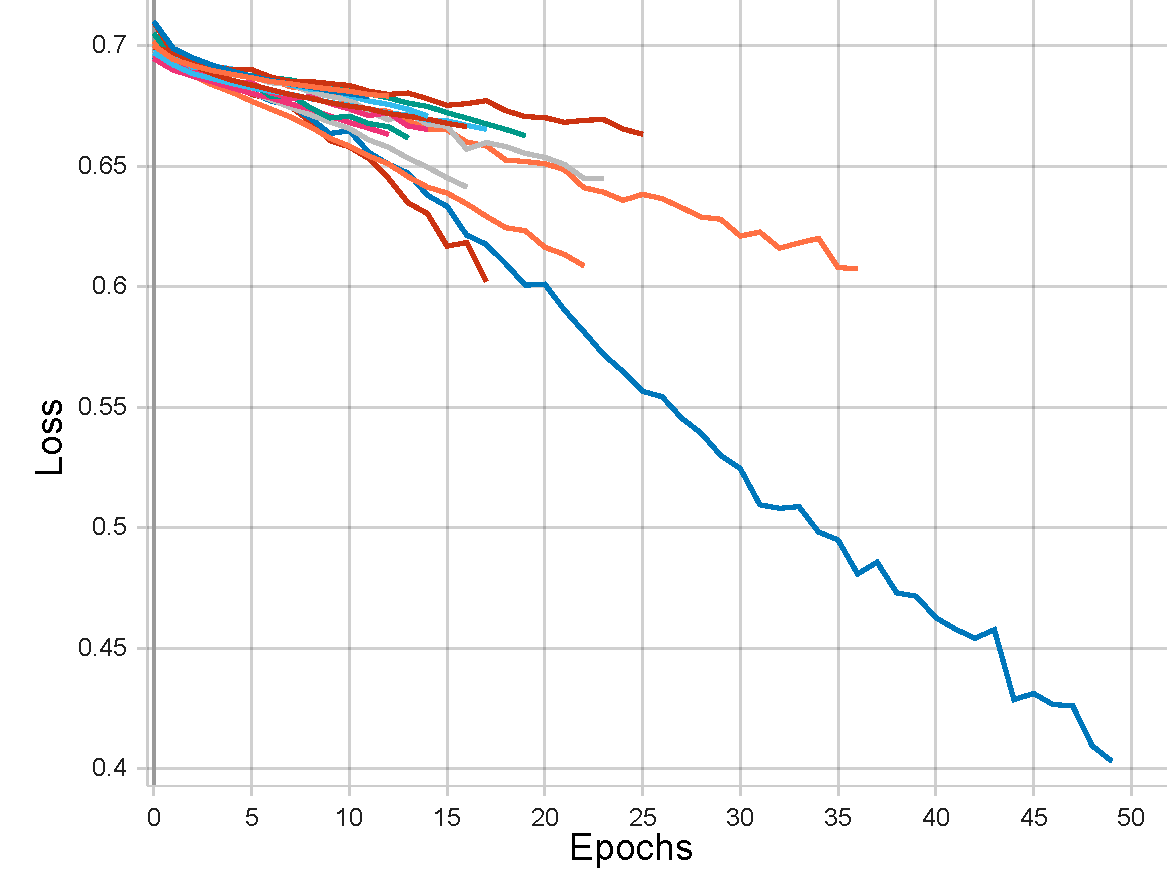
\includegraphics[width=0.95\columnwidth]{figures/results/cnn/cnn_all_loss_t.pdf}
    \caption[Training losses for Iteration 2]{Figure of all training losses of the combinations of Conv1D Layers and Dense Layers in Iteration 2}
    \label{fig:iteration2_train_loss}
\end{figure}
\FloatBarrier

\subsubsection{Validation accuracies and losses}
\begin{figure}[ht]
    \centering
    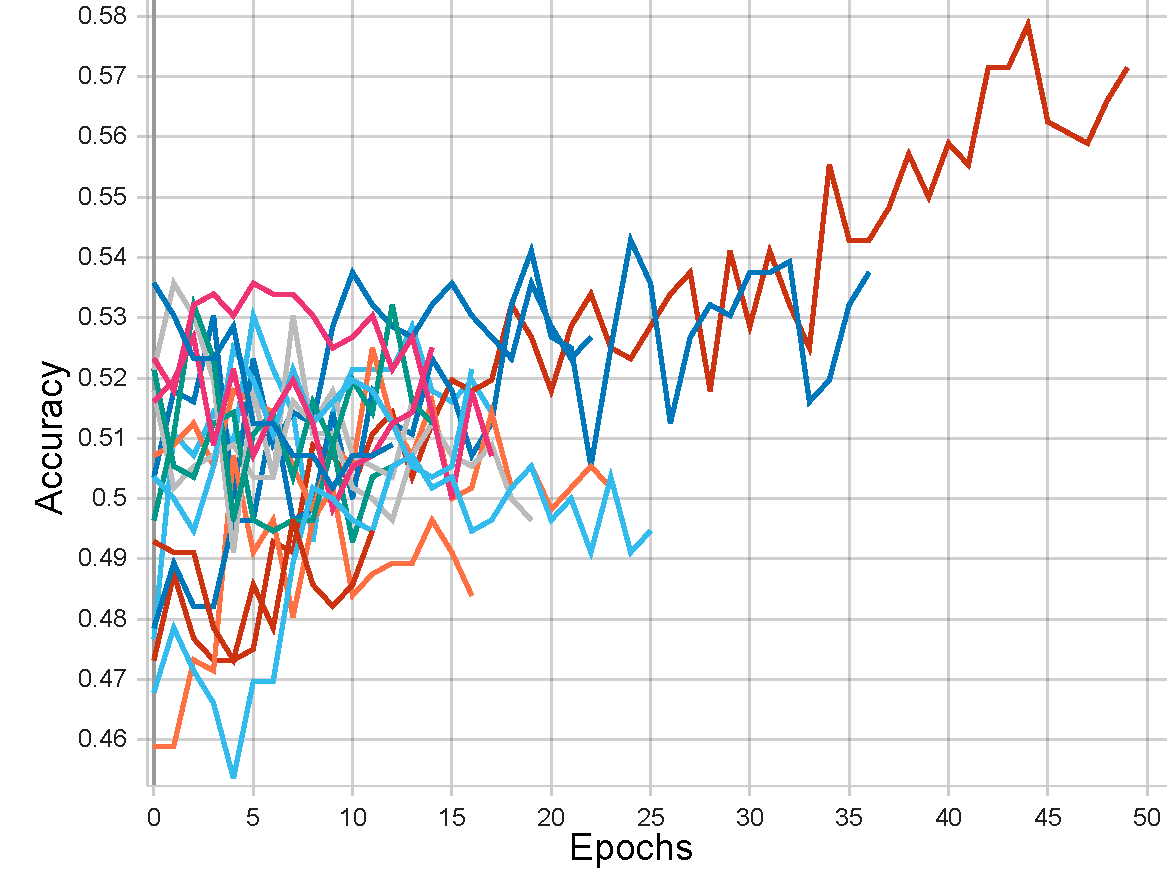
\includegraphics[width=0.95\columnwidth]{figures/results/cnn/cnn_all_acc.pdf}
    \caption[Validation accuracies for Iteration 2]{Figure of all validation accuracies of the combinations of Conv1D Layers and Dense Layers in Iteration 2}
    \label{fig:iteration2_all_accuracy}
\end{figure}
\FloatBarrier
\begin{figure}[ht]
    \centering
    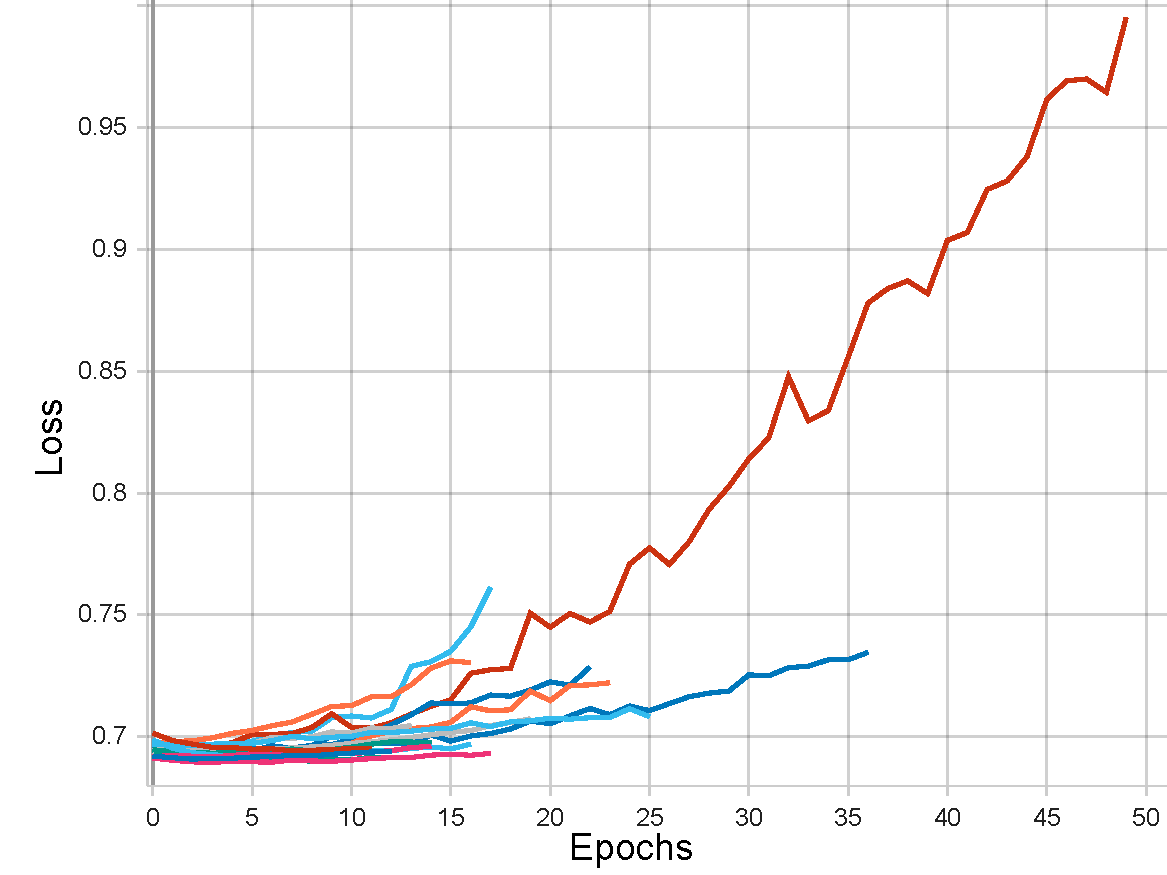
\includegraphics[width=0.95\columnwidth]{figures/results/cnn/cnn_all_loss.pdf}
    \caption[Validation losses for Iteration 2]{Figure of all validation losses of the combinations of Conv1D Layers and Dense Layers in Iteration 2}
    \label{fig:iteration2_all_loss}
\end{figure}
\FloatBarrier

There are varying degrees of success with different combinations of layers; some do not improve in accuracy and others do.
The validation losses using the sparse categorical loss function as described earlier in \autoref{sec:model_fitting}
were used to help identify which models had the lowest error rate; and as an increasing validation
loss is an indicator of overfitting, it was used to filter models showing overfitting.

\subsection{Accuracies of the best result}
\begin{figure}[ht]
    \centering
    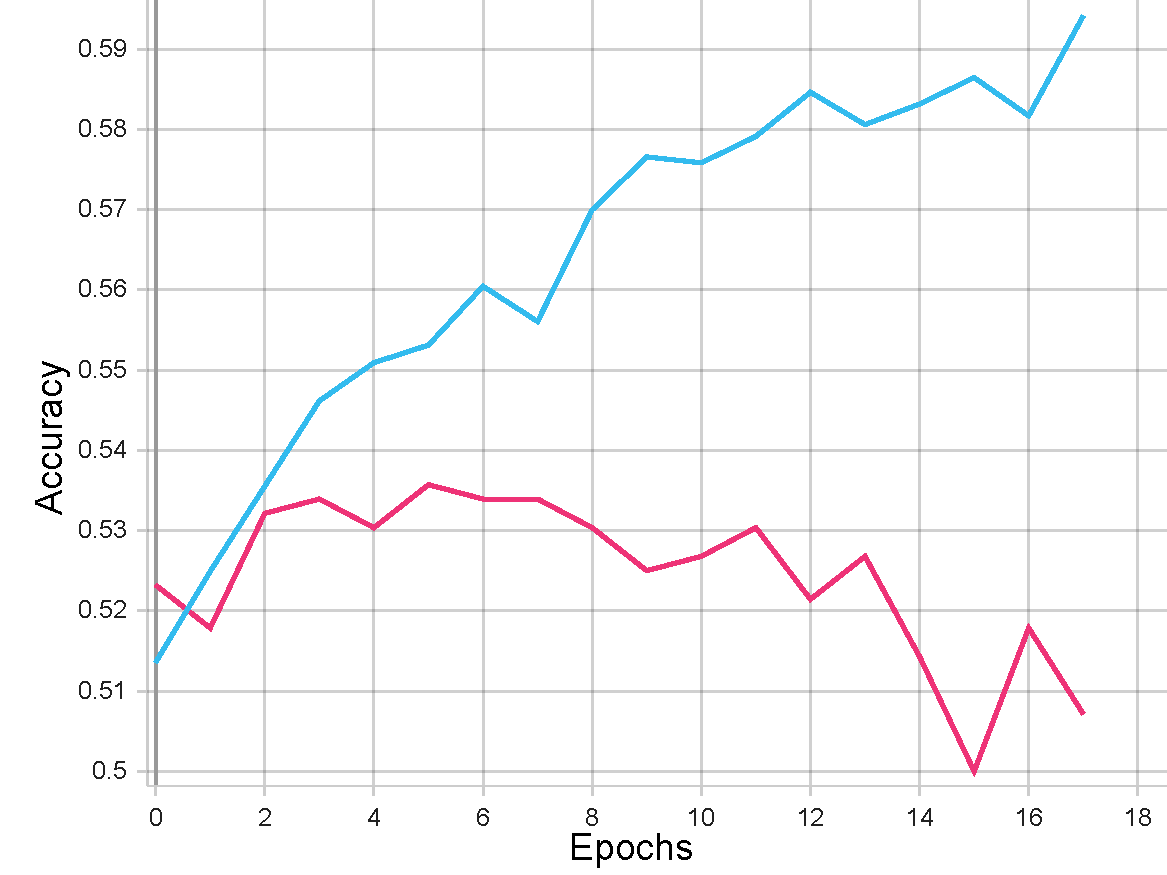
\includegraphics[width=0.95\columnwidth]{figures/results/cnn/cnn_1C32-1D64_acc.pdf}
    \caption[Best accuracy for Iteration 2]{Figure of the best accuracy of the combinations of Conv1D Layers and Dense Layers in Iteration 2}
    \label{fig:iteration2_best_accuracy}
\end{figure}
\FloatBarrier
\begin{figure}[ht]
    \centering
    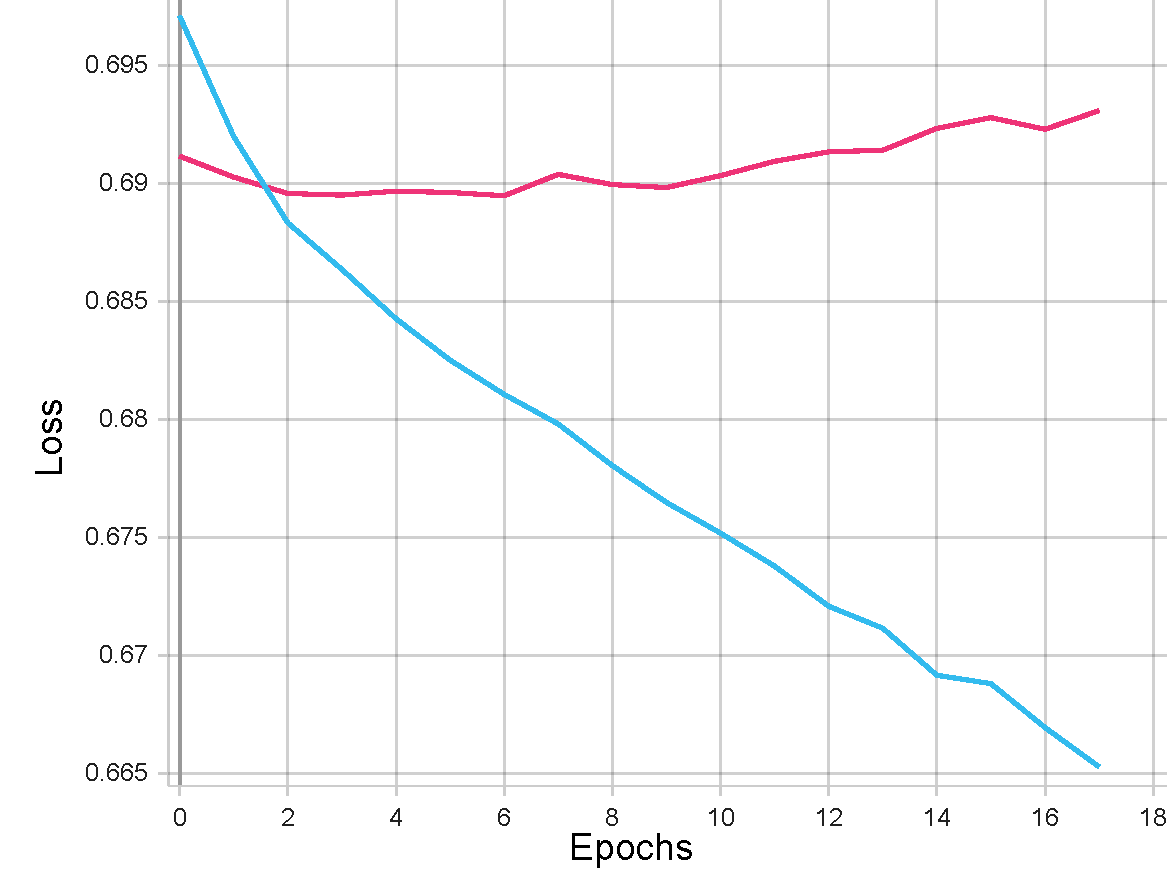
\includegraphics[width=0.95\columnwidth]{figures/results/cnn/cnn_1C32-1D64_loss.pdf}
    \caption[Best loss for Iteration 2]{Figure of the best loss of the combinations of Conv1D Layers and Dense Layers in Iteration 2}
    \label{fig:iteration2_best_loss}
\end{figure}
\FloatBarrier
The best model found within this iteration was one with a one CNN layer of size 32 followed
by the final Dense layer of size 2. The blue line represents the training set and the pink line represents
the validation set. The validation loss shows little overfitting as can be seen in
\autoref{fig:iteration2_best_loss}. At 5 epochs, the validation accuracy reaches its highest value of
53.57\% whilst the training accuracy reached above 55.31\%.
\subsection{Evaluation of iteration 2}
With a validation accuracy above 53\% it suggests that there is only minimal improvement above a random choice. It forms a good
basis for testing further AI models, specifically the CNN-LSTM hybrid model.
There are various limitations with regards to iteration 2. This iteration does not test various combinations of
input features nor does it test various sequence lengths. Furthermore, there could be another number of layers or
layer sizes that is better suited to the problem but unfortunately many have not been tested due to time constraints.

\section{Accuracy of Iteration 3}
As mentioned in \autoref{ssec:iteration3layers}, various combinations of Conv1D layers, LSTM layers and Dense layers were tested,
each with various sizes. The results of all of the models can be seen in \autoref{fig:iteration3_train_accuracy}
and \autoref{fig:iteration3_all_accuracy}.\\
The results of the best model can be seen in \autoref{fig:iteration3_best_accuracy}

\subsection{Accuracies of all tests}
In the charts below, each line represents a combination of different layer types and sizes of the Conv1D, LSTM and Dense layers.
For both the training and validation accuracy charts, each line has a corresponding line in the loss charts with the same colour.
There are 64 lines in total for this iteration as there were 2 Conv1D layer amounts, 2 LSTM layer amounts, 2 Dense layer amounts,
as well as 2 Conv1D layer sizes, 2 LSTM layer sizes and 2 Dense layer sizes in the tests.

\subsubsection{Training accuracies and losses}
\begin{figure}[ht]
    \centering
    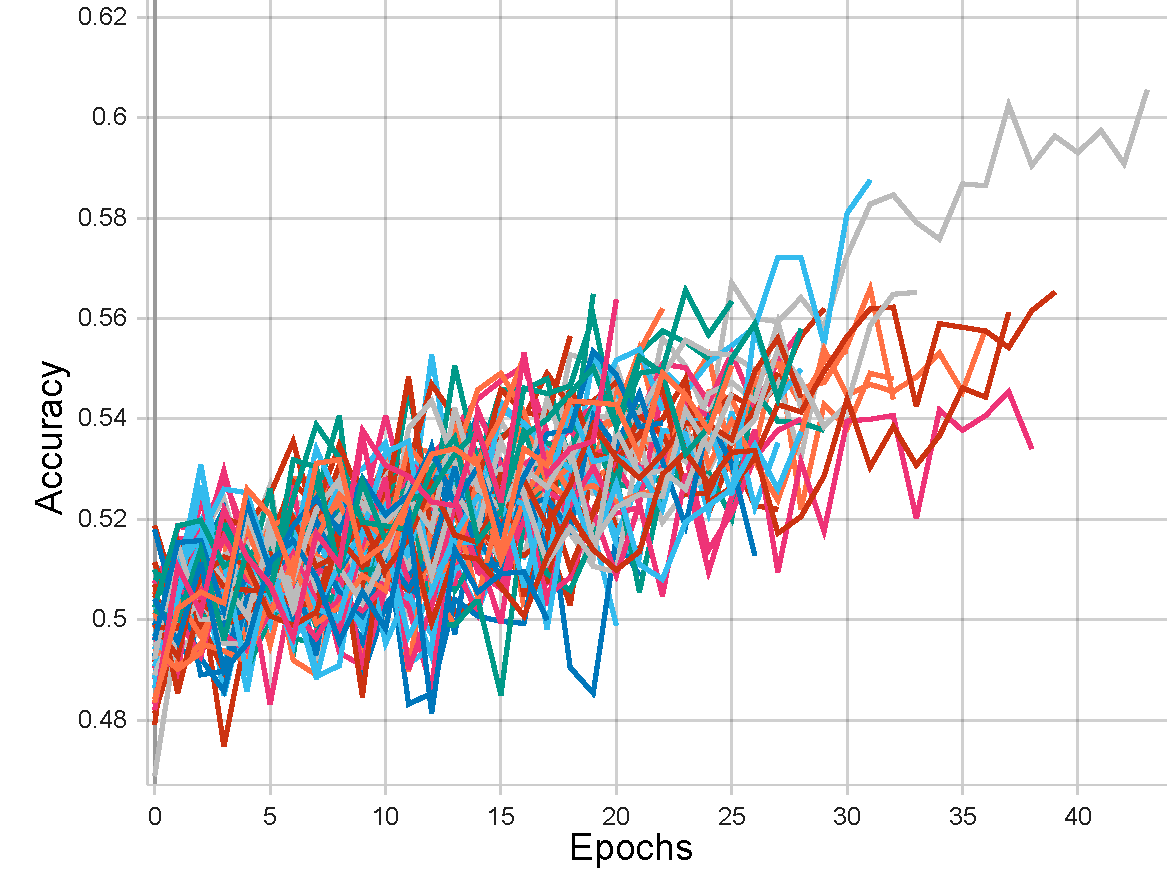
\includegraphics[width=0.95\columnwidth]{figures/results/cnnlstm/cnnlstm_all_acc_t.pdf}
    \caption[Training accuracies for Iteration 3]{Figure of all training accuracies of the combinations of Conv1D, LSTM and Dense Layers in Iteration 3}
    \label{fig:iteration3_train_accuracy}
\end{figure}
\FloatBarrier
\begin{figure}[ht]
    \centering
    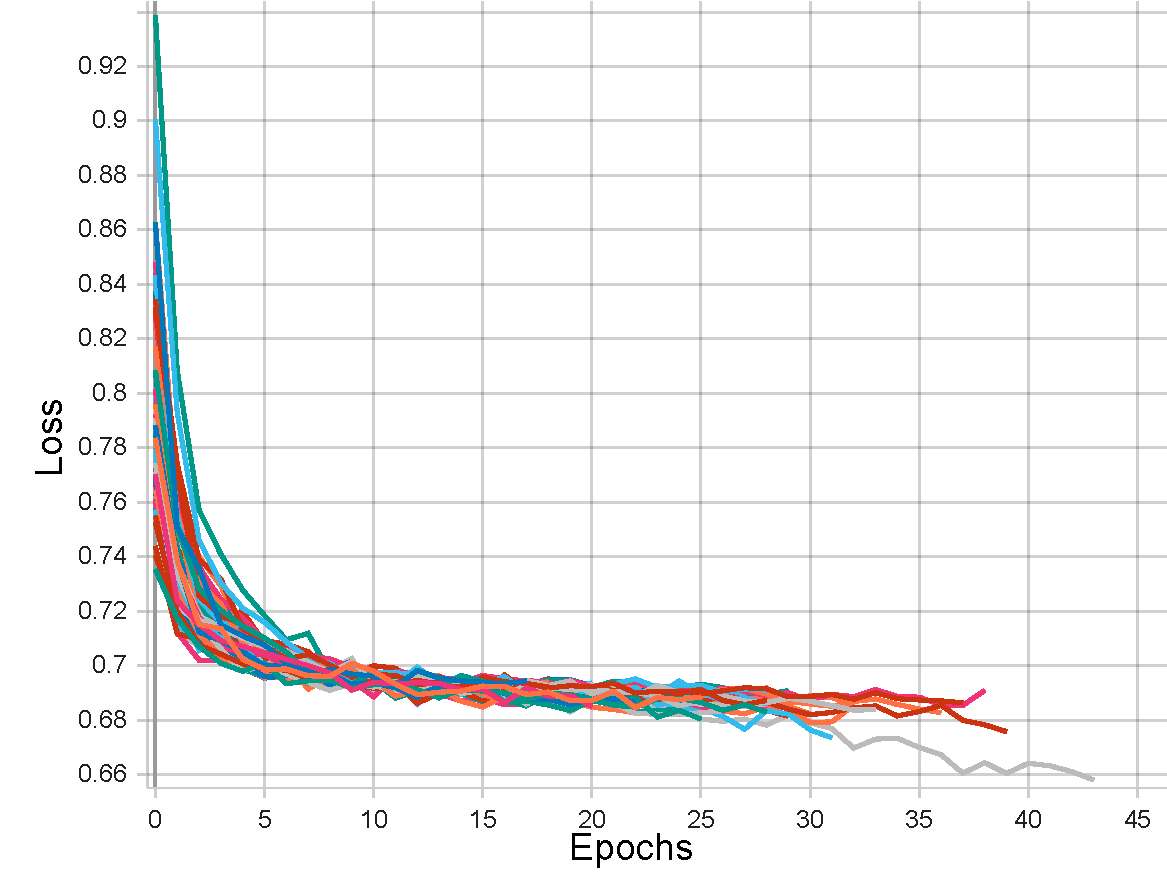
\includegraphics[width=0.95\columnwidth]{figures/results/cnnlstm/cnnlstm_all_loss_t.pdf}
    \caption[Training losses for Iteration 3]{Figure of all training losses of the combinations of Conv1D, LSTM and Dense Layers in Iteration 3}
    \label{fig:iteration3_train_loss}
\end{figure}
\FloatBarrier

\subsubsection{Validation accuracies and losses}
\begin{figure}[ht]
    \centering
    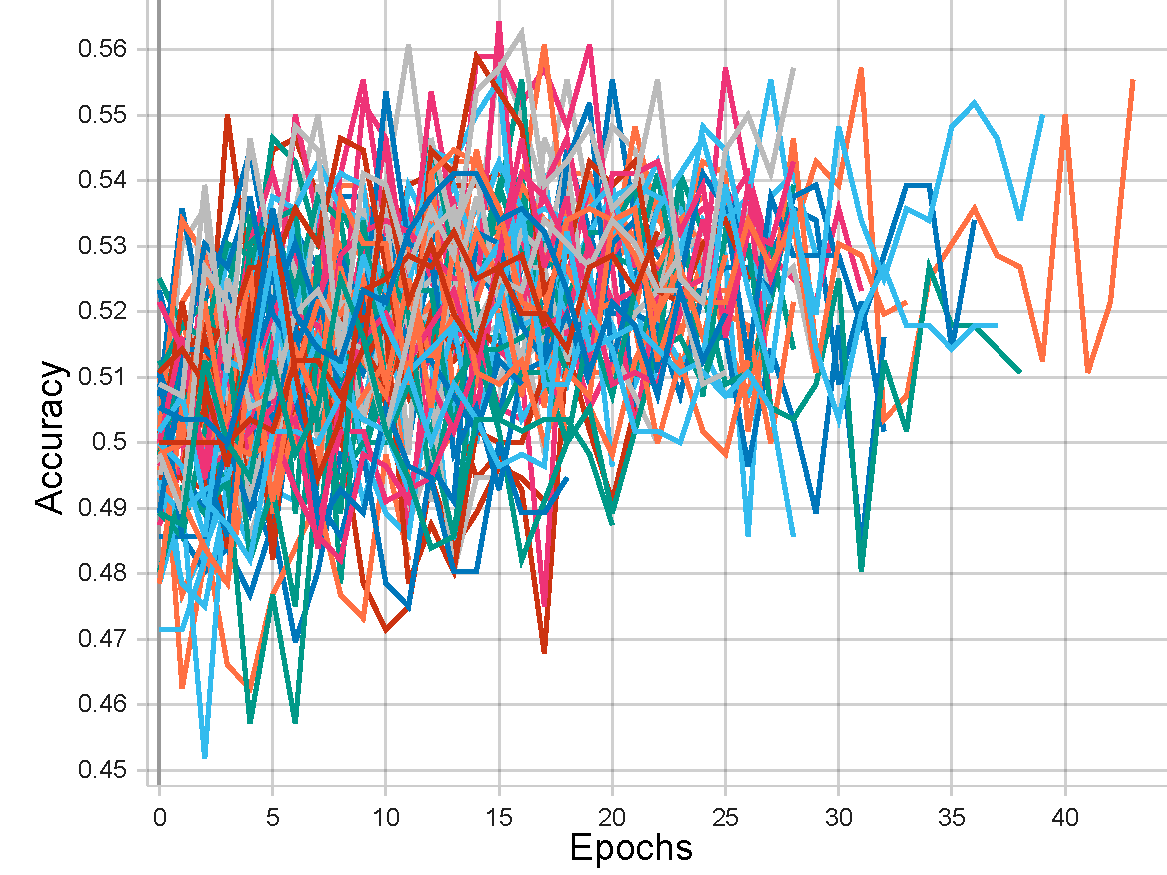
\includegraphics[width=0.95\columnwidth]{figures/results/cnnlstm/cnnlstm_all_acc.pdf}
    \caption[Validation accuracies for Iteration 3]{Figure of all validation accuracies of the combinations of Conv1D, LSTM and Dense Layers in Iteration 3}
    \label{fig:iteration3_all_accuracy}
\end{figure}
\FloatBarrier
\begin{figure}[ht]
    \centering
    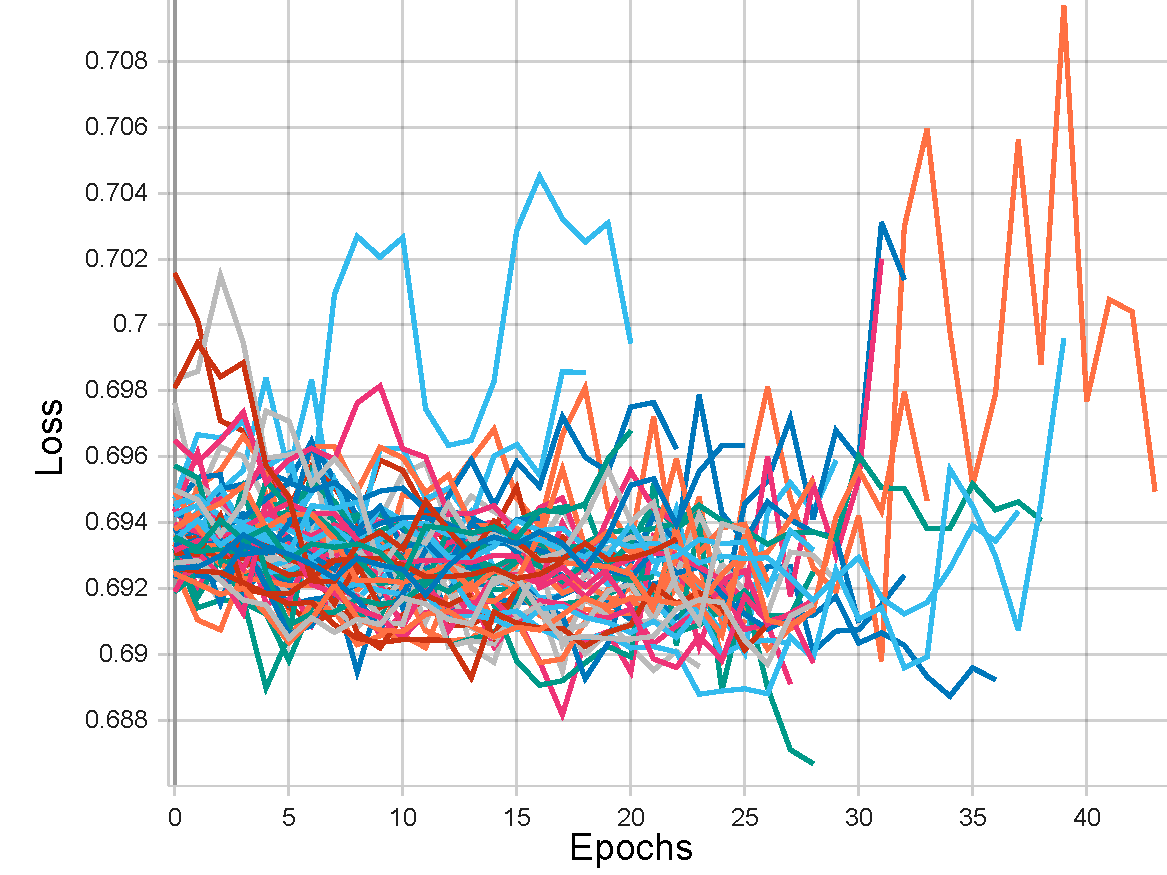
\includegraphics[width=0.95\columnwidth]{figures/results/cnnlstm/cnnlstm_all_loss.pdf}
    \caption[Validation losses for Iteration 3]{Figure of all validation losses of the combinations of Conv1D, LSTM and Dense Layers in Iteration 3}
    \label{fig:iteration3_all_loss}
\end{figure}
\FloatBarrier

There are varying degrees of success with different combinations of layers; some do not improve in accuracy and others do.
The validation losses using the sparse categorical loss function as described earlier in \autoref{sec:model_fitting}
were used to help identify which models had the lowest error rate; and as an increasing validation
loss is an indicator of overfitting, it was used to filter models showing overfitting.

\subsection{Accuracies of the best result}
\begin{figure}[ht]
    \centering
    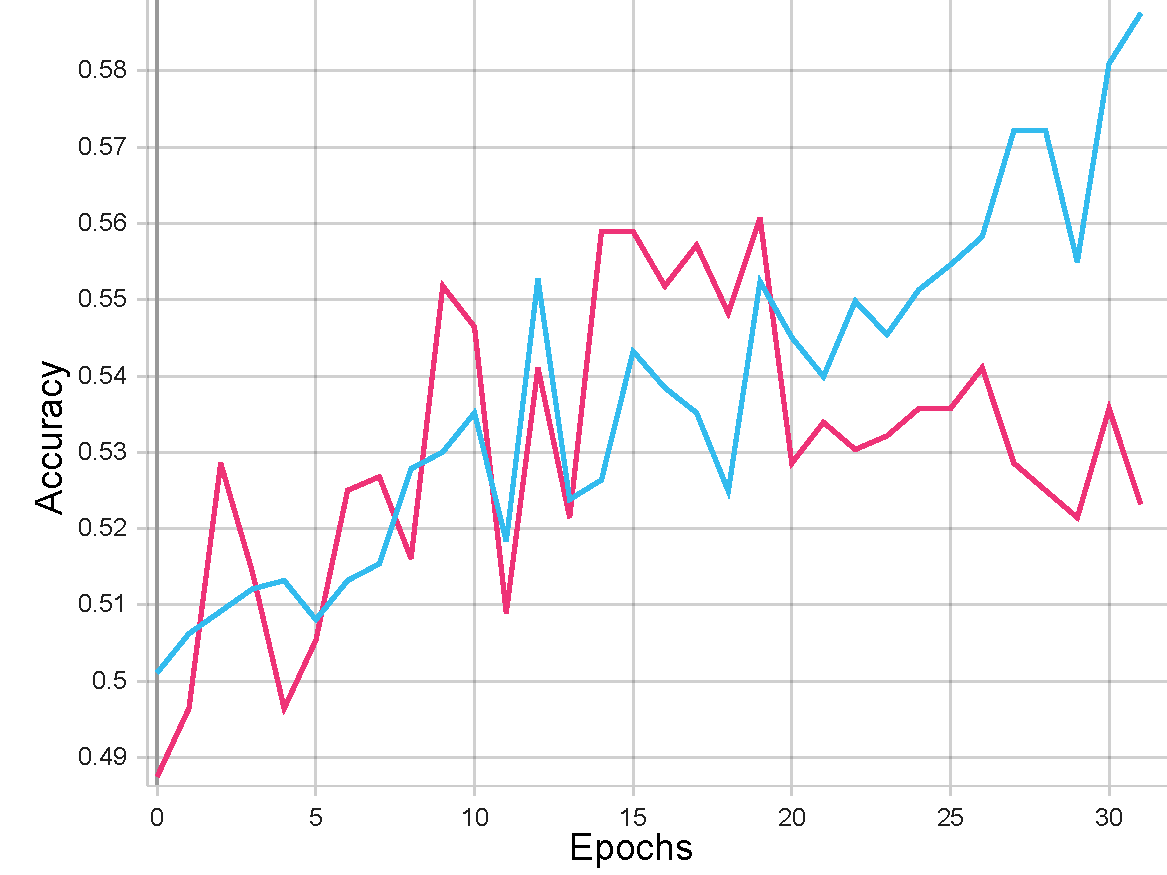
\includegraphics[width=0.95\columnwidth]{figures/results/cnnlstm/cnnlstm_2C32-1L16-2D64_acc.pdf}
    \caption[Best accuracy for Iteration 3]{Figure of the best accuracy of the combinations of Conv1D, LSTM and Dense Layers in Iteration 3}
    \label{fig:iteration3_best_accuracy}
\end{figure}
\FloatBarrier
\begin{figure}[ht]
    \centering
    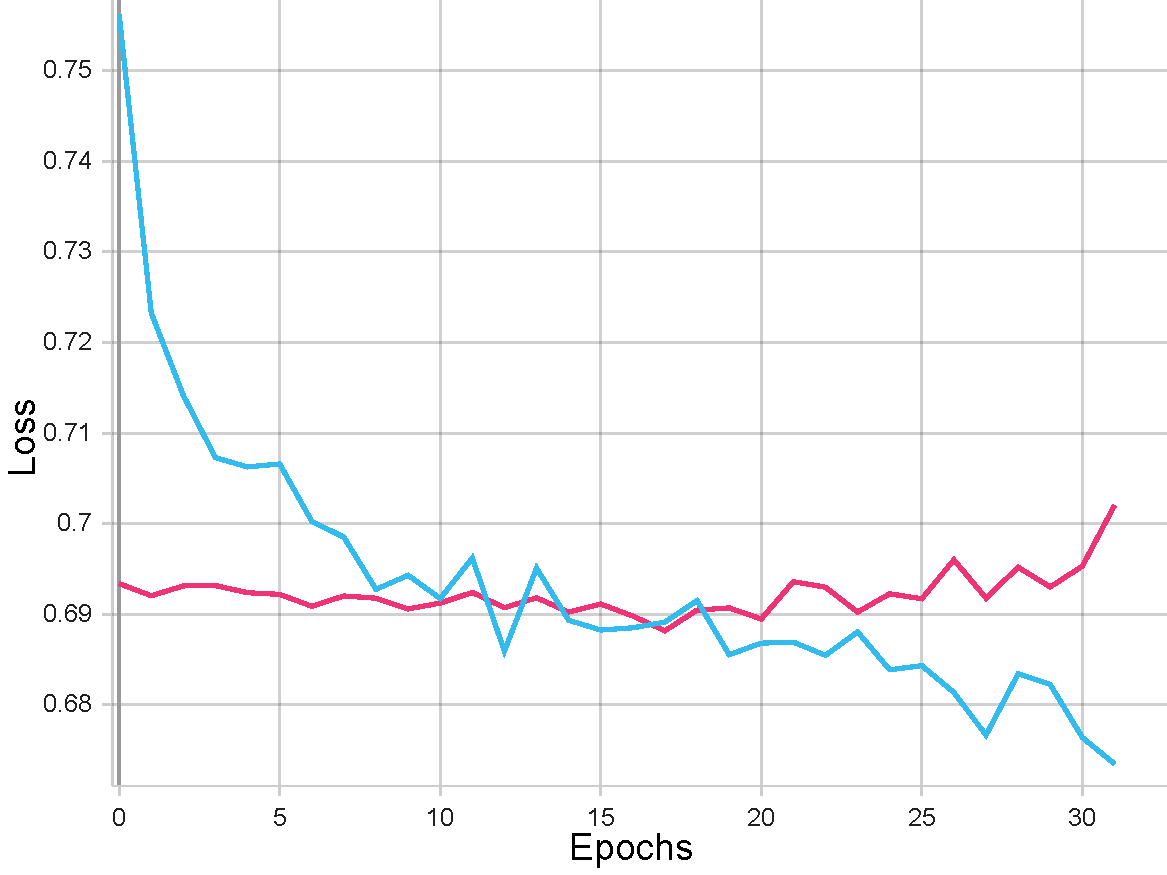
\includegraphics[width=0.95\columnwidth]{figures/results/cnnlstm/cnnlstm_2C32-1L16-2D64_loss.pdf}
    \caption[Best loss for Iteration 3]{Figure of the best loss of the combinations of Conv1D, LSTM and Dense Layers in Iteration 3}
    \label{fig:iteration3_best_loss}
\end{figure}
\FloatBarrier
The best model found within this iteration was one with a two Conv1D layers of size 32 followed by 1 LSTM layer
of size 16, and a Dense layer of size 64 followed by a the final Dense layer of size 2.
The blue line represents the training set and the pink line represents
the validation set. The validation loss shows little overfitting as can be seen in
\autoref{fig:iteration3_best_loss}. At 19 epochs, the validation accuracy reaches its highest value of
56.07\% whilst the training accuracy reached 55.24\%. The validation accuracy being somewhat greater than the
training accuracy can be explained by the dropout layers within the model that can affect the results of the training
set but does not affect the validation set.
\subsection{Evaluation of iteration 3}
With a validation accuracy above 56.07\%, it is currently the best model when compared to the previous iterations.
This suggests there is a significant advantage compared to randomly guessing the next trading day's direction.
Furthermore, this aligns with the studies analysed in the literature review. However, this iteration alone cannot be
used to answer the research questions as it does not test different sequence lengths or combinations of input features.
Additionally, there could be different number of layers or sizes of layers that perform better but unfortunately could
not be tested due to time constraints.